\chapter{DBCASE 2.0}
\begin{figure}[H]
    \centering
    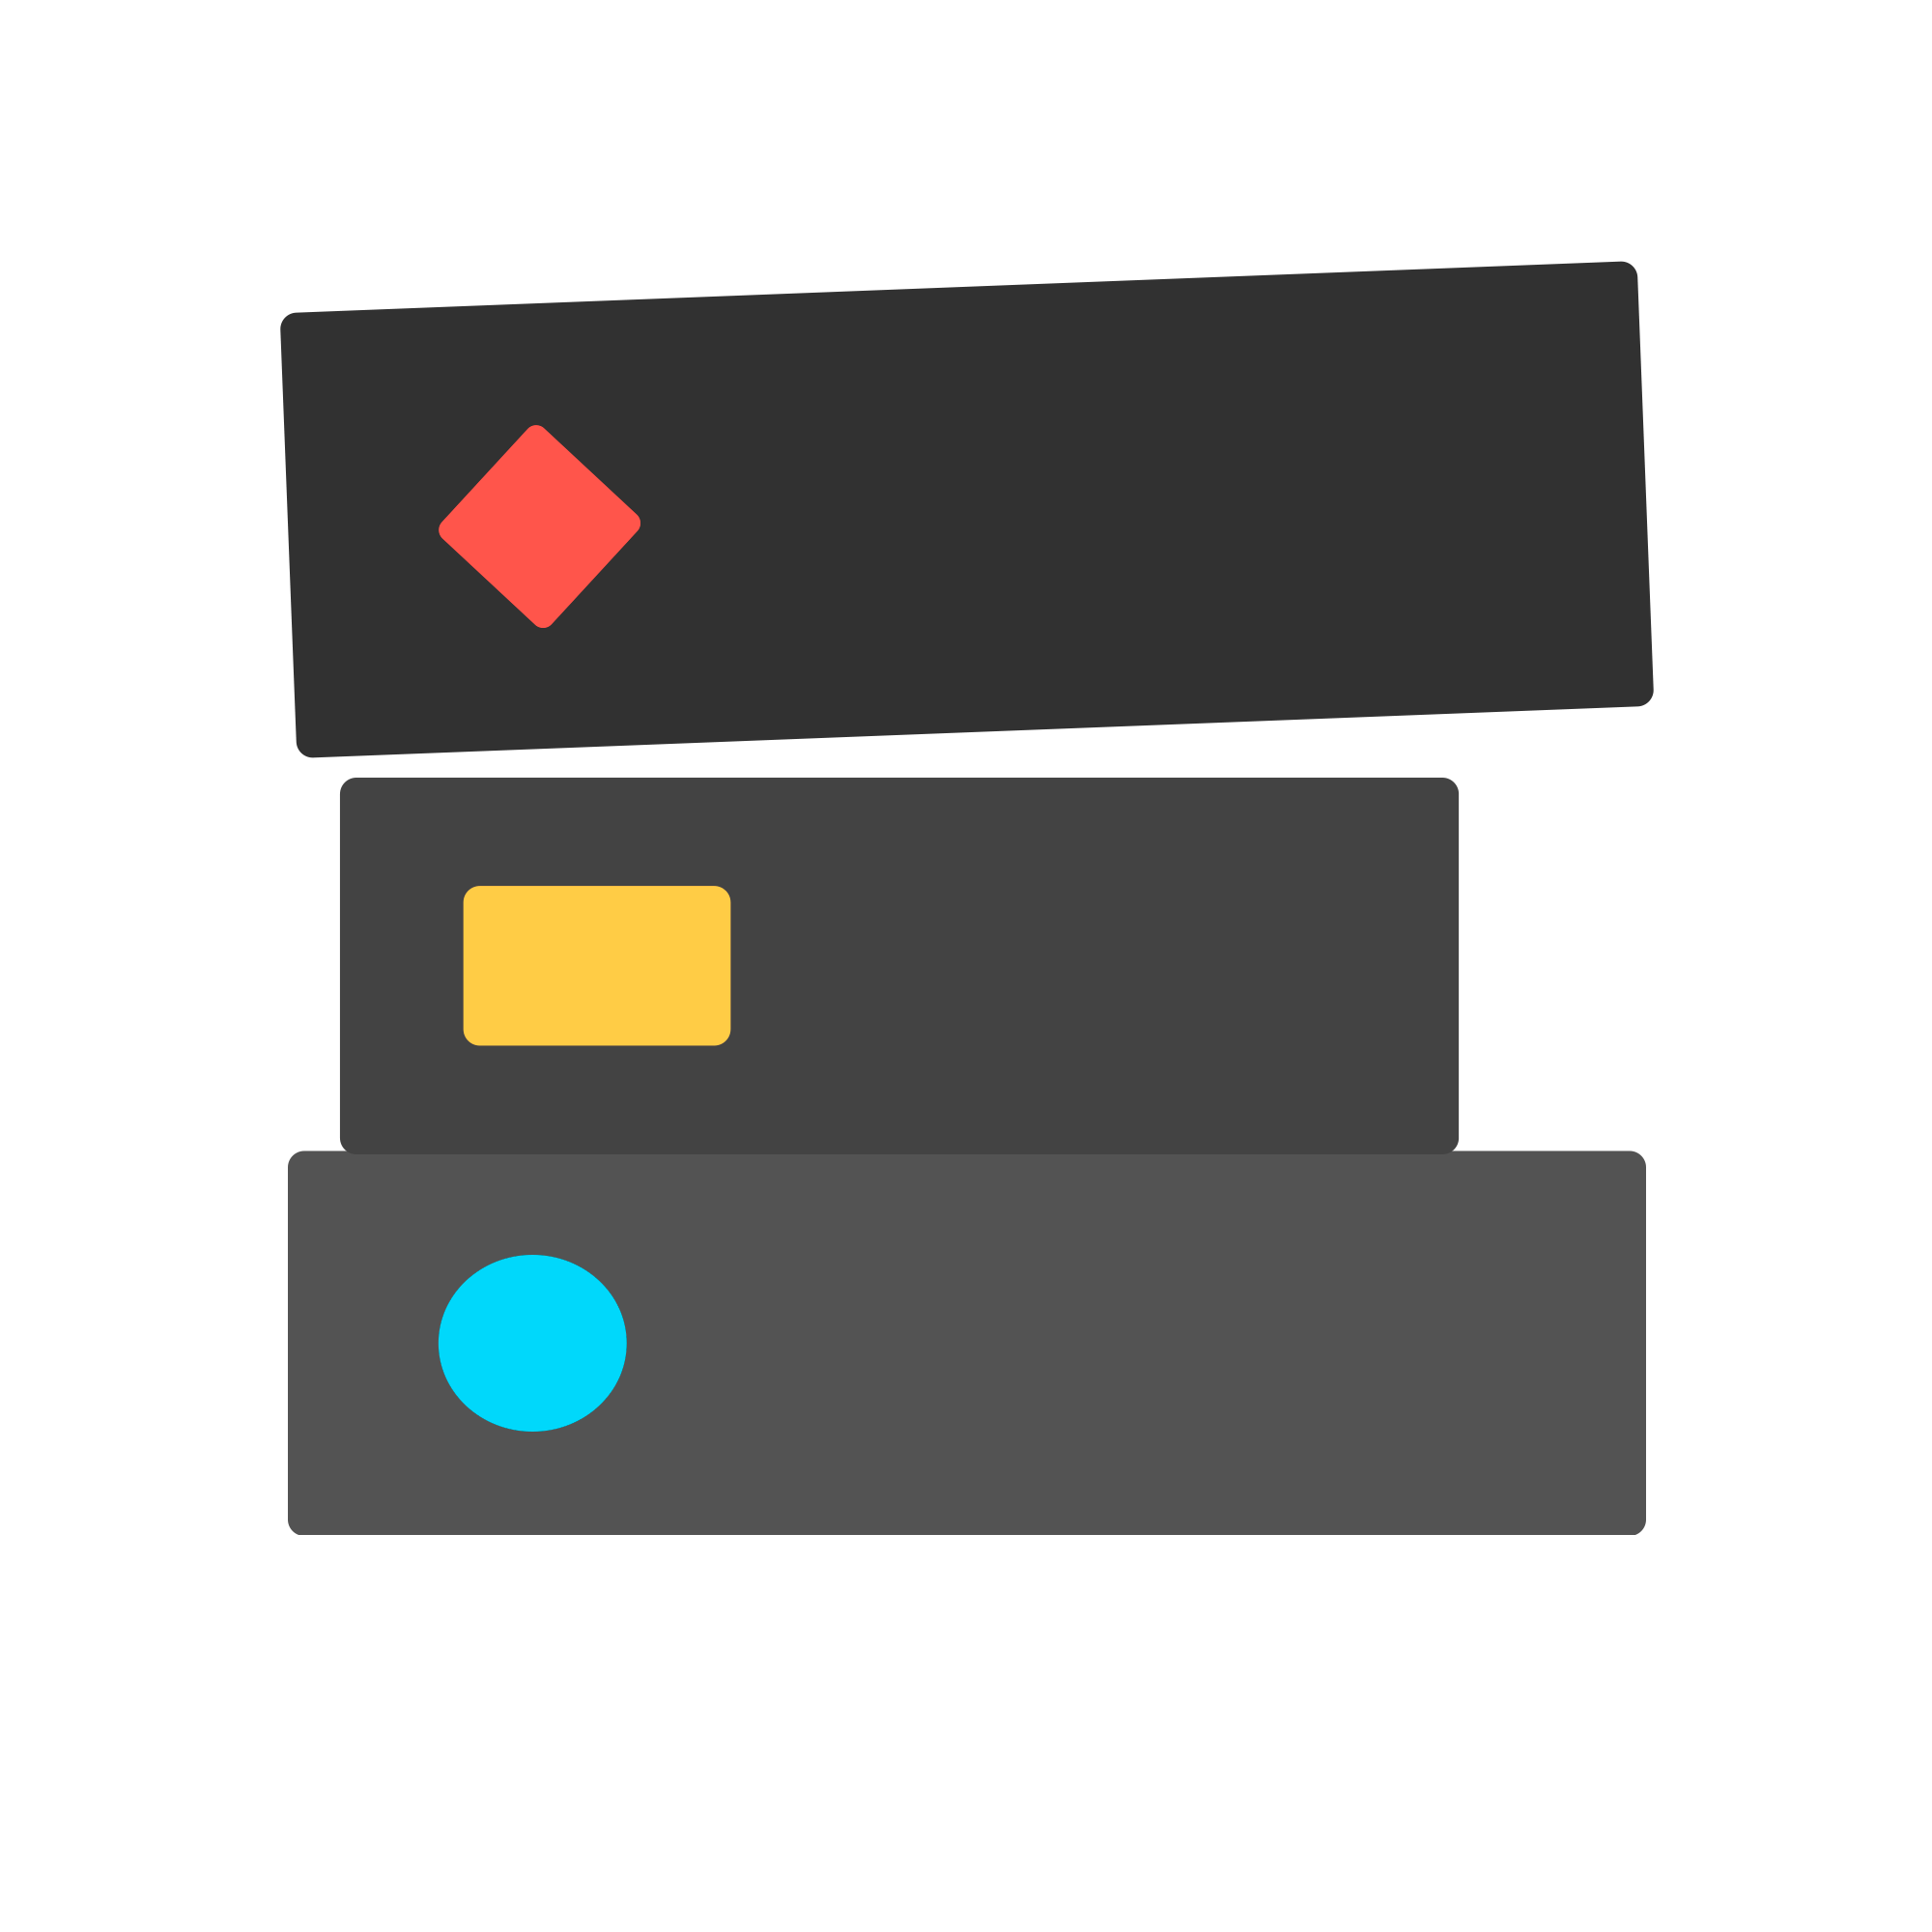
\includegraphics[width=0.5\textwidth]{img/DBCase_logo.png}
\end{figure}
%%
\section{Introducción}
DBCASE 2.0 surge como una actualización al proyecto DBCASE con la que se pretende dar un nuevo aspecto al diseño de la interfaz de usuario y continuar con la implementación de nuevas funcionalidades.\\

El programa está destinado principalmente al uso académico y por ello ha sido pensado como una herramienta didáctica que ayude al alumno en su proceso de aprendizaje, aunque también puede ser usada profesionalmente como una manera fácil y rápida de construir una base de datos relacional. Por ello la herramienta permite al usuario crear una base de datos funcional a partir de un diagrama sin necesidad de que conozca ningún lenguaje de programación de base de datos, lo que es perfecto para alumnos que se estén iniciando en la materia.\\

La herramienta está desarrollada utilizado el lenguaje de programación Java. También cuenta con elementos creados mediante html y css.

%%
\subsection{Motivación}
Dado que el uso de las bases de datos relacionales está ampliamente extendido, desde hace años existen herramientas pensadas para la creación de una base de datos a partir del diseño de un diagrama, simplificando el proceso.\\

DBCase pretende centrarse en el proceso de aprendizaje del diseño y creación de una bases de datos, llevando al usuario a través de todas las fases e informándole de los errores que puede tener su diseño. Por ello DBCase está pensada especialmente para ser utilizada en un ámbito académico diferenciándola así de otras alternativas disponibles.\\


\subsection{Antecedentes}
El proyecto DBCase 2.0 es la continuación de dos proyectos anteriores.\\

\textbf{DBDT} de sistemas informáticos (2007/2008)\\

El proyecto fue el punto de partida de la aplicación. Pretendía dar una alternativa al diseño de bases de datos en papel, enfocándose en el ámbito académico. Se realizó un programa multiplataforma optando por el lenguaje java.\\

Autores del proyecto:
\begin{itemize}
    \item Alberto Milán Gutierrez, Miguel Martinez Segura, Francisco Javier Cáceres González
    \item Profesora Directora: Yolanda García Ruiz
\end{itemize}

\textbf{DBCase} de sistemas informáticos (2008/2009)\\

Este proyecto supuso una ampliación y mejora de las funcionalidades que ofrecía el proyecto del año anterior, se mejoró el diseño del diagrama entidad relación y creo la posibilidad de traducir el diagrama a código soportado por distintos gestores de bases de datos. \\

Autores del proyecto:
\begin{itemize}
    \item Rodrigo Denis Cepeda Mateos, Cristina Marco de Francisco, Tello Serrano Gordillo
\end{itemize}
El proyecto servía como una herramienta bastante útil, pero que debido al paso de los años había quedado algo obsoleta. Sobre todo en lo que respecta a su interfaz gráfica.
%%
\subsection{Objetivos}
El principal objetivo del proyecto era rehabilitar la aplicación para su uso académico en las aulas, para ello se establecieron los siguientes objetivos.
\begin{itemize}
    \item Actualizar el diseño de la interfaz gráfica de la aplicación, haciéndola más usable y moderna.
    \begin{itemize}
        \item Cambiar la disposición de los paneles, de manera que el flujo de trabajo de la aplicación resulte más simple e intuitivo.
        \item Rediseñar el panel de códigos, separando el modelo lógico del físico y simplificando el reporte de errores y advertencias.
        \item Mejorar la representación del diagrama entidad relación.
    \end{itemize}
    \item Corregir los posibles errores que arrastrase la aplicación desde versiones anteriores y continuar añadiendo funcionalidades nuevas.
    \begin{itemize}
        \item Completar la traducción al modelo lógico, añadiendo indicaciones para que el usuario entienda cómo se ha realizado.
        \item Añadir la posibilidad de escoger un tema oscuro para la interfaz gráfica.
    \end{itemize}
\end{itemize}
